\section{Introdução ao magnetismo e aos ímãs}

\frame{
	\frametitle{Eletromagnetismo}
	\begin{block}{História}
		Durante muito tempo, acreditou-se que \textbf{eletricidade} e \textbf{magnetismo} eram o mesmo fenômeno. Foi somente em 1600 que o médico e físico inglês Gilbert escreveu um livro distinguindo as duas teorias. Apesar dessa diferenciação entre os dois fenômenos, havia fortes indícios de que existia alguma relação entre eles.
	\end{block}
}

\frame{
	\frametitle{Eletromagnetismo}
	\begin{block}{Qual é a relação entre Eletricidade e Magnetismo?}
		Um físico dinamarquês chamado \textbf{Hans Christian Oesterd} descobriu em 1820 que toda \textbf{corrente elétrica gera um campo magnético}. \\
	\end{block}
}

\frame{
	\frametitle{Eletromagnetismo}
	\begin{block}{Aplicação}
		A partir dessa descoberta, foi possível termos os aparelhos e máquinas que usamos hoje.
		\begin{itemize}
			\item O liquidificador, barbeadora e furadeira têm como elemento básico o \textbf{motor elétrico}. Vários outros aparelhos, como, o gerador elétrico, transformador e detectores de metais funcionam pelo princípio do \textbf{eletromagnetismo}.
		\end{itemize}
	\end{block}
}

\frame{
	\frametitle{Eletromagnetismo}
	\centerline{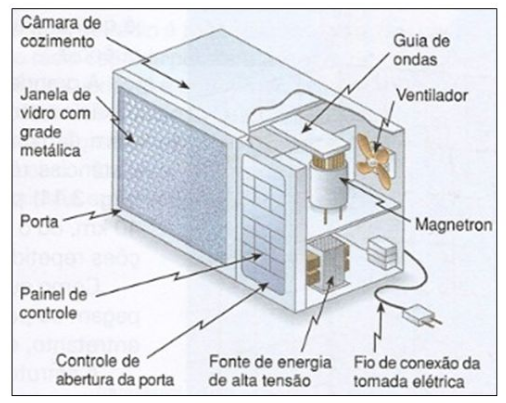
\includegraphics[width=0.45\linewidth]{Figuras/Ch06/fig1.PNG}}
	\begin{block}{Aplicação}
		\begin{itemize}
			\item O magnetron recebe, de um transformador, uma tensão fixa de cerca de 400 volts e gera dentro do aparelho ondas eletromagnéticas de \SI{2450}{\giga\hertz}, a mesma freqüência de ressonância das moléculas de água. Essas ondas são refletidas várias vezes nas paredes metálicas do forno sobre o alimento, fazendo vibrar as moléculas de água contidas nele. A fricção entre elas produz calor, cozinhando o alimento.
		\end{itemize}
	\end{block}
}

\frame{
	\frametitle{Eletromagnetismo}
	\centerline{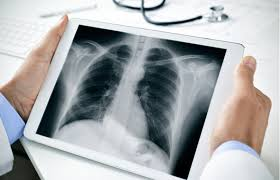
\includegraphics[width=0.55\linewidth]{Figuras/Ch06/fig2.jpg}}
	\begin{block}{Aplicação}
		\begin{itemize}
			\item Na radiografia o corpo é bombardeado por raios-X, que são um tipo de onda eletromagnética. Os raios-X sofrem interação com o corpo, e depois, de certa maneira, essa interação é analisada para a formação da imagem.
		\end{itemize}
	\end{block}
}

\frame{
	\frametitle{Magnetismo}
	\begin{block}{Definição}
		O magnetismo é uma área da física que estuda a \textbf{atração} e \textbf{repulsão} de objetos magnéticos.
		\begin{itemize}
			\item Sabe-se que o magnetismo não é algo novo, uma vez que desde o século VII a.C. já eram utilizados seus conceitos; textos gregos apontam para a existência do magnetismo, \textbf{propriedade} de corpos presentes numa região denominada “Magnésia” e daí surgiu o nome da propriedade de atração e repulsão de determinados corpos.
			\item Tales de Mileto, filósofo, físico e matemático grego (623 a.C. - 558 a.C.) foi quem observou a \textbf{atração do ímã natural}, a magnetita, com o ferro.
		\end{itemize}
	\end{block}
}

\frame{
	\frametitle{Magnetismo}
	\begin{block}{ímã}
		O \textbf{ímã} pode representar esse estudo e é todo material que produz um \textbf{campo magnético}.
		\begin{itemize}
			\item Existem os ímãs naturais, que são rochas com propriedades magnéticas, como a magnetita.
			\item Existem também ímãs artificiais, criados por ligas metálicas, como as de níquel-cromo.
		\end{itemize}
	\end{block}
	\centerline{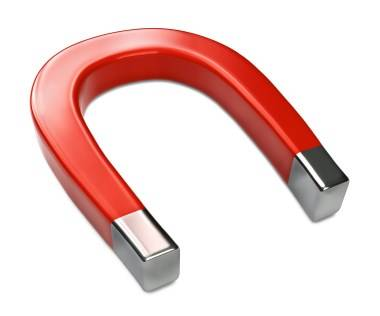
\includegraphics[width=0.4\linewidth]{Figuras/Ch06/fig3.jpeg}}
}

\frame{
	\frametitle{Magnetismo}
	\centerline{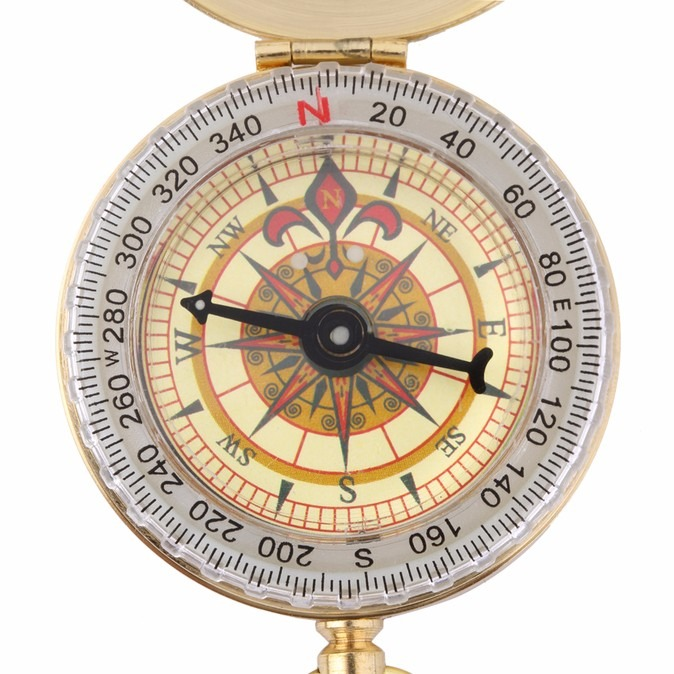
\includegraphics[width=0.4\linewidth]{Figuras/Ch06/fig4.jpg}}
	\begin{block}{Aplicação}
		A primeira aplicação prática do magnetismo foi encontrada pelos chineses: a \textbf{bússola}, que se baseia na interação do \textbf{campo magnético de um ímã} (a agulha da bússola) com o campo magnético terrestre.
	\end{block}
}

\frame{
	\frametitle{Propriedades dos ímãs}
	\begin{block}{Polos de um ímã}
		A bússola é um ímã, assim como a Terra. Todo ímã tem um \textbf{polo norte} e outro \textbf{sul}, sendo que os \textbf{opostos se atraem}. Logo, o polo norte magnético da bússola (ponteiro pintado) aponta para o polo sul magnético do planeta que, por coincidência, está perto do polo norte geográfico da Terra.
	\end{block}
	\centerline{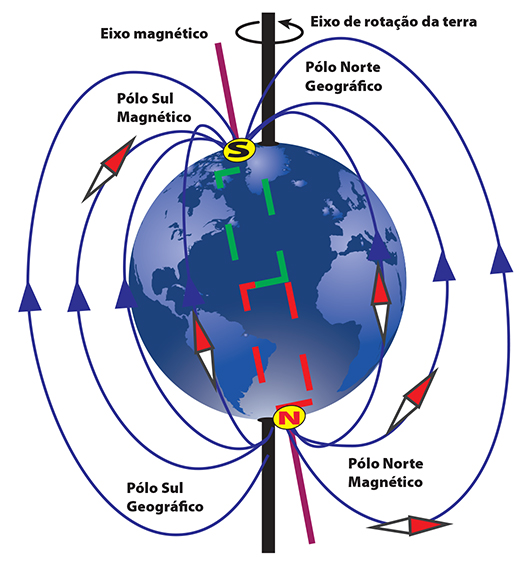
\includegraphics[width=0.4\linewidth]{Figuras/Ch06/fig5.png}}
}

\frame{
	\frametitle{Propriedades dos ímãs}
	\begin{block}{Ação entre polos}
		Aproximando-se do polo norte de um ímã o polo sul de outro ímã, nota-se uma atração. A partir da figura abaixo, podemos enunciar a lei da força magnética: \textbf{polos da mesma natureza se repelem e de naturezas diferentes se atraem}.
	\end{block}

	\bigskip

	\newcommand{\barmagsn}{\filldraw[fill=blue,draw=black,thin] (0,0) rectangle ++(1,-0.5); \node[right, white, thick] at (0,-0.25) {S}; \filldraw[fill=red,draw=black,thin] (1,0) rectangle ++(1,-0.5); \node[left,white,thick] at (2,-0.25) {N};}
	\newcommand{\barmagns}{\filldraw[fill=red,draw=black,thin] (0,0) rectangle ++(1,-0.5); \node[right, white, thick] at (0,-0.25) {N}; \filldraw[fill=blue,draw=black,thin] (1,0) rectangle ++(1,-0.5); \node[left,white,thick] at (2,-0.25) {S};}
	
	\begin{minipage}{0.49\linewidth}
		\centering
		\begin{tikzpicture}[x=1cm,y=1cm]
			\barmagsn
			\node (nMag) at (4,-0.25) {\begin{tikzpicture}[x=1cm,y=1cm]
				\barmagns
				\end{tikzpicture}};
			
			\draw[{Latex[length=0.4cm,width=0.2cm]}-,thick] (1,-1) -- (1.8,-1);
			\draw[-{Latex[length=0.4cm,width=0.2cm]},thick] (3.2,-1) -- (4,-1);
		\end{tikzpicture}
		\medskip
		
		Repulsão
	\end{minipage}
	\hfill
	\begin{minipage}{0.49\linewidth}
		\centering
		\begin{tikzpicture}[x=1cm,y=1cm]
			\barmagsn
			\node (nMag) at (4,-0.25) {\begin{tikzpicture}[x=1cm,y=1cm]
				\barmagsn
				\end{tikzpicture}};
			
			\draw[-{Latex[length=0.4cm,width=0.2cm]},thick] (1,-1) -- (1.8,-1);
			\draw[{Latex[length=0.4cm,width=0.2cm]}-,thick] (3.2,-1) -- (4,-1);
		\end{tikzpicture}
	\medskip
	
	Atração	
	\end{minipage}
	
%	\centerline{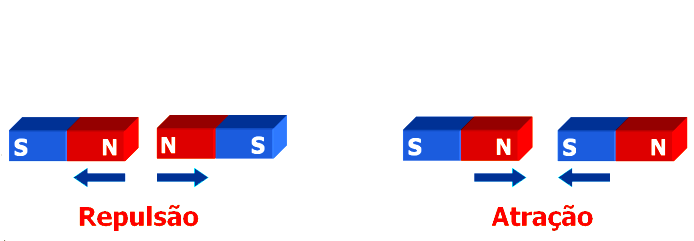
\includegraphics[width=0.8\linewidth]{Figuras/Ch06/fig6.png}}
}

\frame{
	\frametitle{Propriedades dos ímãs}
	\begin{block}{Inseparabilidade dos polos}
		Os polos de um ímã são \textbf{inseparáveis}. Não é possível partir um ímã em duas partes para separar o polo norte do polo sul. Serrando-se um ímã transversalmente, obtêm-se \textbf{dois novos ímãs completos}, isto é, surgem na secção de corte polos contrários aos das respectivas extremidades.
	\end{block}

	\newcommand{\barmagns}{\filldraw[fill=red,draw=black,thin] (0,0) rectangle ++(1,-0.5); \node[right, white, thick] at (0,-0.25) {N}; \filldraw[fill=blue,draw=black,thin] (1,0) rectangle ++(1,-0.5); \node[left,white,thick] at (2,-0.25) {S};}
	
	\centering
	\begin{tikzpicture}[]
		\barmagns
		\node (nMag1) at (0,-1) {\begin{tikzpicture}[x=1cm,y=2cm]
			\barmagns
			\end{tikzpicture}};
		\node (nMag2) at (2,-1) {\begin{tikzpicture}[x=1cm,y=2cm]
			\barmagns
			\end{tikzpicture}};
		\node (nMag11) at (-0.5,-1.75) {\begin{tikzpicture}[x=0.5cm,y=2cm]
			\barmagns
			\end{tikzpicture}};
		\node (nMag21) at (0.5,-1.75) {\begin{tikzpicture}[x=0.5cm,y=2cm]
			\barmagns
			\end{tikzpicture}};
		\node (nMag12) at (1.5,-1.75) {\begin{tikzpicture}[x=0.5cm,y=2cm]
			\barmagns
			\end{tikzpicture}};
		\node (nMag22) at (2.5,-1.75) {\begin{tikzpicture}[x=0.5cm,y=2cm]
			\barmagns
			\end{tikzpicture}};
	\end{tikzpicture}

%	\centerline{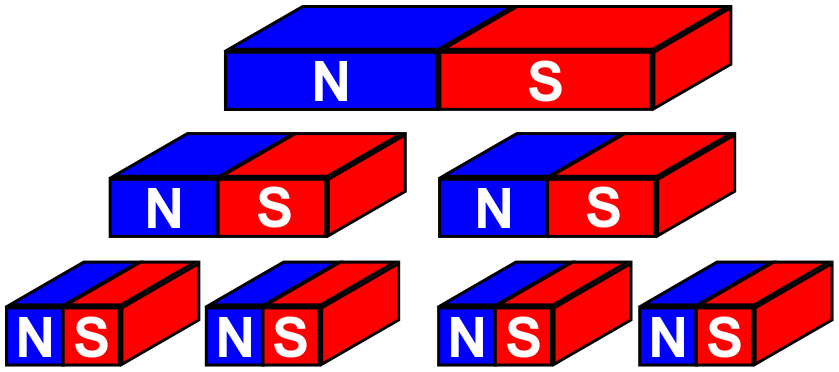
\includegraphics[width=0.6\linewidth]{Figuras/Ch06/fig7.png}}
}

\frame{
	\frametitle{Campo magnético de um ímã}
	\begin{block}{Definição}
		Um ímã gera no espaço ao seu redor um \textbf{campo magnético} que tem a propriedade de interagir com outros corpos. \textbf{O campo magnético de um ímã é a parte que envolve o ímã}.
		\begin{itemize}
			\item Para medir a ação de um ímã, associamos, a cada ponto do campo, uma grandeza \textbf{vetorial} denominada \textbf{vetor indução magnética} ou simplesmente vetor campo magnético, representado por $\vec{B}$.
		\end{itemize}
	\end{block}
}

\frame{
	\frametitle{Campo magnético de um ímã}
	\begin{block}{Linhas de indução}
		As linhas que tangenciam o vetor $\vec{B}$ em cada ponto são denominadas \textbf{linhas de indução} (análogas às linhas de força existentes no campo elétrico).
		\begin{itemize}
			\item Por convenção, as linhas de indução do campo magnético \textbf{partem do polo norte para o polo sul}. Se pensarmos em fechar uma das linhas de indução, o ímã irá ficar no interior das linhas, possuindo um único sentido, onde \textbf{dentro do ímã a orientação será de sul para norte}.
		\end{itemize}
	\end{block}
	
	\centering
	\scalebox{0.8}{
		\begin{tikzpicture}[x=1cm,y=1cm,directed/.style={postaction={decorate,decoration={markings,
					mark=at position .1 with {\arrowreversed[scale=1.5]{stealth}},
					mark=at position .9 with {\arrowreversed[scale=1.5]{stealth}}}}},
		directedDash/.style={postaction={decorate,decoration={markings,
					mark=at position .1 with {\arrow[scale=1.5]{stealth}},
					mark=at position .9 with {\arrow[scale=1.5]{stealth}}}}},
		tangent/.style={postaction={decorate,decoration={markings, mark=at position .7 with {\draw[ultra thick,stealth-,green!60!black,solid](-12pt,0)node[above]{$\vec{B}$}--(12pt,0);}}}},
		tangentDash/.style={postaction={decorate,decoration={markings, mark=at position .7 with {\draw[ultra thick,stealth-,green!60!black,solid](12pt,0)--node[below left,rotate=180]{$\vec{B}$}(-12pt,0);}}}},
		fLines/.style={thick,dashed,directed,tangent},
		fLinesDash/.style={thick,dashed,directedDash,tangentDash},
		]
		\def\lmag{1.8}  % length of magnet
		\def\wmag{0.4}  % thickness of magnet
		\def\nc{5}      % no. of lines = 2*\nc+1
		
		\begin{scope}
		\coordinate (A) at (-\lmag/2,\wmag/2);
		\coordinate (B) at (\lmag/2,-\wmag/2);
		\draw[fill, color=blue](A) rectangle ++(\lmag/2,-\wmag)node[white,midway]{S};
		\draw[fill, color=red](0,-\wmag/2) rectangle ++(\lmag/2,\wmag)node[white,midway]{N};
		
		\clip (-4,-2) rectangle (4,2);
		\foreach \r in {1,...,\nc}{
			\draw[fLines]($(A)-(0,0.5*\r*\wmag/\nc)$) arc(({270-asin(\lmag/(2*\r))}):({-90+asin(\lmag/(2*\r))}):\r);
			\draw[fLinesDash]($(B)+(0,0.5*\r*\wmag/\nc)$) arc(({90-asin(\lmag/(2*\r))}):({-270+asin(\lmag/(2*\r))}):\r); }
		\draw[fLines] (-\lmag/2,0) -- ++(-6,0);
		\draw[fLines] (\lmag/2,0) ++(6,0)--(\lmag/2,0);
		\end{scope}
		\end{tikzpicture}
	}
	
%	\centerline{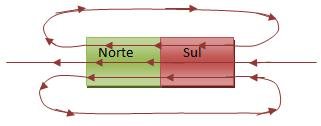
\includegraphics[width=0.7\linewidth]{Figuras/Ch06/fig9.jpg}}
}

\frame{
	\frametitle{Campo magnético de um ímã}
	\begin{block}{Linhas de indução - \textbf{Importante}}
		Lembre-se que as \textbf{linhas de indução} mostram somente a \textbf{direção e o sentido}. Para que possamos medir a \textbf{intensidade} de um campo, usa-se o \textbf{vetor indução magnética}, que é representado por $\vec{B}$.
	\end{block}
}

\section*{Exercícios}
\frame{
	\frametitle{Exercícios}
	\begin{block}{}
		01. Explique a tirinha abaixo. \\
		\vspace{0.2cm}
		\centerline{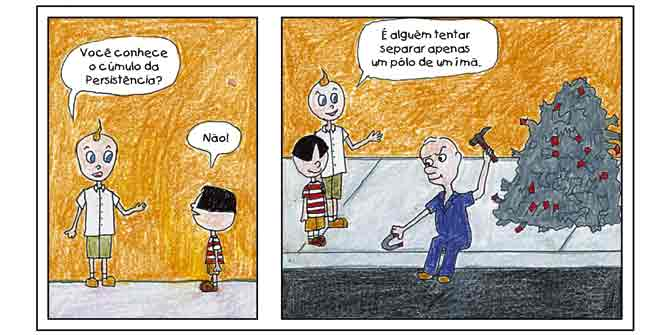
\includegraphics[width=0.95\linewidth]{Figuras/Ch06/fig8.png}}
	\end{block}
}

\section*{Referências}
\frame{
	\frametitle{Referências e Exercícios Complementares}
	\begin{itemize}
		\item ALEXANDRE, Charles K.; SADIKU, Matthew N. O. Fundamentos de Circuitos Elétricos. 5. ed. Porto Alegre: AMGH, 2013.
	\end{itemize}
	%\centering{\alert{Página 36 - \textbf{1.6.1 até 1.6.5, 1.6.17 até 1.6.19}}} \\
	\centering{\alert{Lista de exercícios 06}}
}


